\documentclass[10pt, a4paper, twoside]{basestyle}

\usepackage[backend=biber,firstinits=true,maxnames=100,style=alphabetic,maxalphanames=4,doi=true,isbn=false,url=false,eprint=true]{biblatex}
\bibliography{bibliography}

\usepackage[Mathematics]{semtex}
\usepackage{chngcntr}
\counterwithout{equation}{section}

%%%% Shorthands.

%%%% Title and authors.

\title{%
\textdisplay{%
On an Article by Celledoni et al.%
}%
}
\author{Pascal~Leroy (phl)}
\begin{document}
\maketitle
\begin{sloppypar}
\noindent
This document provides clarifications, corrections, and accuracy improvements to the formul{\ae} presented in \cite{Celledoni2007}.  It follows the notation
and conventions of that paper.  Note that the preprint \cite{Celledoni2007} differs in some of the formul{\ae} from the final publication \cite{Celledoni2008},
and that we follow the former because the latter introduced errors.
\end{sloppypar}

\section*{Preamble}
We remind the reader of the derivation formul{\ae} for the Jacobian elliptic functions (\cite{NistHMF2010}, section 22.13(i)):
\[
\begin{dcases}
\derivop{u}{\JacobiSN u} &= \JacobiCN u \JacobiDN u \\
\derivop{u}{\JacobiCN u} &= -\JacobiSN u \JacobiDN u \\
\derivop{u}{\JacobiDN u} &= -k^2 \JacobiSN u \JacobiCN u
\end{dcases}
\]
and for the hyperbolic functions (\cite{NistHMF2010}, section 4.34):
\[
\begin{dcases}
\derivop{u}{\HyperbolicTangent u} &= \HyperbolicSecant^2 u \\
\derivop{u}{\HyperbolicSecant u} &= -\HyperbolicSecant u \HyperbolicTangent u
\end{dcases}
\]

\section*{The equations of motion}
We start by writing equation (1) of \cite{Celledoni2007} in coordinates.  The coordinates of $\vm$ and $\VectorSymbol{I}$ are defined by:
\[
\vm\DefineAs
\begin{pmatrix}
m_1 \\ m_2 \\ m_3
\end{pmatrix}
\]
and:
\[
\VectorSymbol{I}\DefineAs
\begin{pmatrix}
I_1 & 0 & 0 \\ 0 & I_2 & 0 \\ 0 & 0 & I_3
\end{pmatrix}
\]
with $I_1 \leq I_2 \leq I_3$.

Euler's equation $\TimeDerivative{\vm} = \commutator{\vm}{\VectorSymbol{\gw}}$ can be written in coordinates in the principal axes frame:
\[
\TimeDerivative{\vm} =
\begin{pmatrix}
m_1 \\ m_2 \\ m_3
\end{pmatrix}
\times
\begin{pmatrix}
m_1/I_1 \\ m_2/I_2 \\ m_3/I_3
\end{pmatrix}
\]
thus:
\begin{equation}
\begin{dcases}
\TimeDerivative{m}_1 &= m_2 m_3 \pa{1/I_3 - 1/I_2}\\
\TimeDerivative{m}_2 &= m_3 m_1 \pa{1/I_1 - 1/I_3}\\
\TimeDerivative{m}_3 &= m_1 m_2 \pa{1/I_2 - 1/I_1}
\end{dcases}
\label{eqneuler}
\end{equation}
\section*{Solution of Euler's equation}
The solution of Euler's equation has three cases depending on the initial value of $\vm$ (more precisely, on the sign of
$\gD_2 = m_1^2 \frac{I_{12}}{I_1} + m_3^2 \frac{I_{32}}{I_3}$, see discussion below).  Figure~\ref{figm} illustrates the 
possible evolutions of $\vm$. The sphere is the surface $\norm\vm = G$, which is an invariant of motion.  The planes are
the surfaces $\gD_2 = 0$ and separate different modes of the motion.
The blue curve is called case (i) in \cite{Celledoni2007}: $\vm$ follows a periodic curve, and when that curve is close to the $m_1$
axis we have a classical case of precession.  The red curve is case (ii), and again the motion of $\vm$ is periodic and exhibits 
precession when the curve remains close to the $m_3$ axis.  The green curve is case (iii): $\vm$ takes an infinite amount
of time to reach the point $\tuple{0, G, 0}$; furthermore, the motion is unstable as any perturbation moves it either to
the blue or the red region where $\vm$ oscillates between points close to $\tuple{0, G, 0}$ and $\tuple{0, -G, 0}$; this is 
the Джанибеков effect.
\begin{figure}[htb!]
\centering
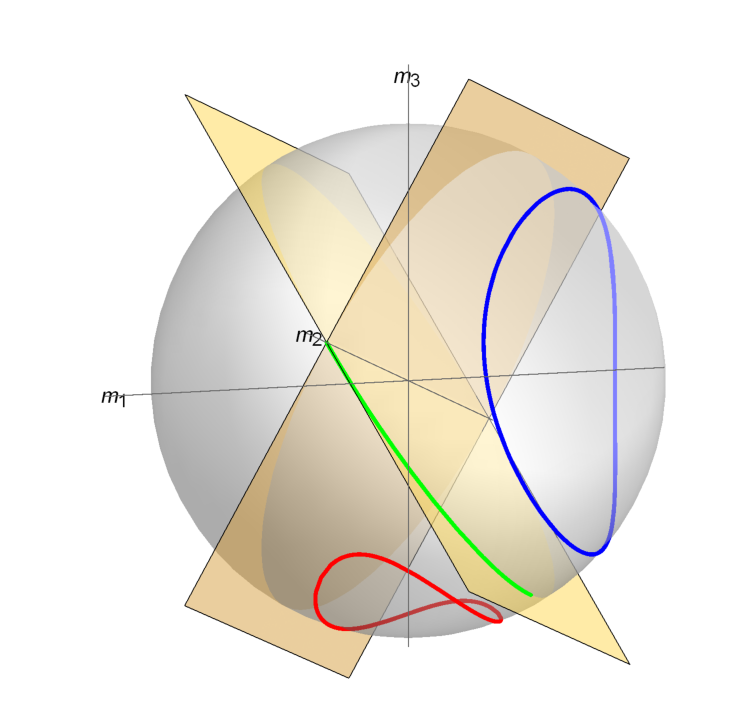
\includegraphics[scale=0.45]{Celledoni-m}
\caption{Possible trajectories of $\vm$: the blue and red curves are cases (i) and (ii), respectively, and correspond to motion
with precession.  The green curve is the (unstable) case (iii) and any perturbation demonstrates the Джанибеков effect.\label{figm}}
\end{figure}

The solutions may also be visualized by intersecting the sphere $\norm\vm = 1$ with ellipsoids defined by the value of the kinetic energy $T$,
which is also a constant of motion.  Since $T = \frac{G^2 - \gD_2}{2 I_2}$, different values of $T$ determine the same modes as above.
\begin{figure}[htb!]
\centering
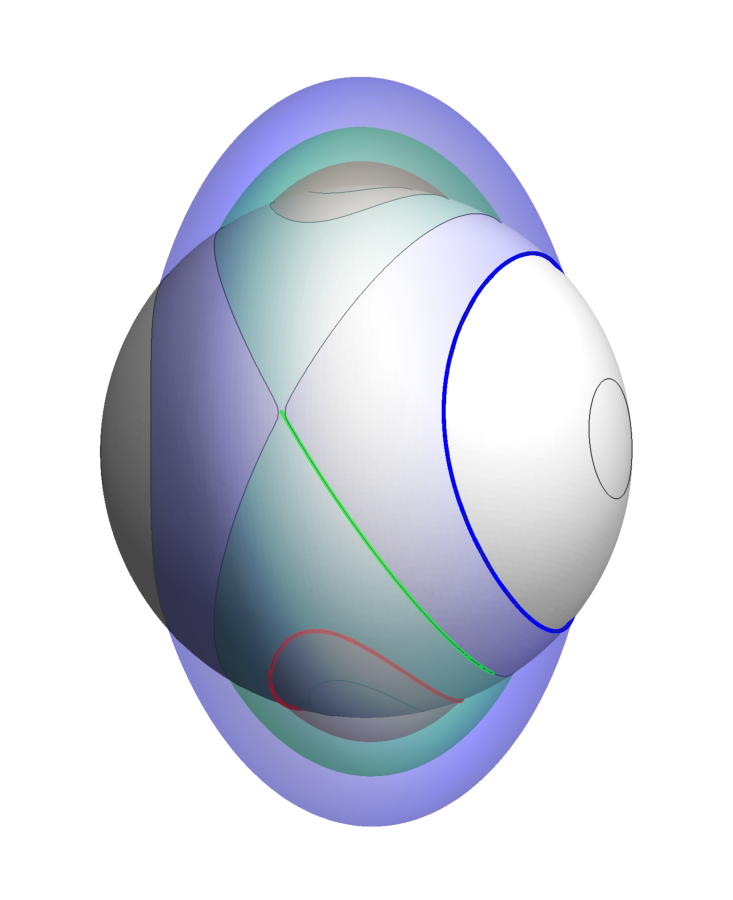
\includegraphics[scale=0.45]{Celledoni-G-T}
\caption{Possible trajectories of $\vm$: the sphere is identical to that of Figure~\ref{figm}.
The ellipsoids are surfaces of equal kinetic energy and intersect the sphere on the blue, red, and green curves depending on the
value of $T$ .\label{figGT}}
\end{figure}

In the rest of this section, we derive (corrected) formul{\ae} for the three cases described above.
\subsection*{Case (i)}
Case (i) of the solution of Euler's equation in section 2.2 of \cite{Celledoni2007} is:
\[
{\vm}_t =
\begin{pmatrix}
\gs B_{13} \JacobiDN\of{\gl t - \gn, k} \\
-B_{21} \JacobiSN\of{\gl t - \gn, k} \\
B_{31} \JacobiCN\of{\gl t - \gn, k}
\end{pmatrix}
\]
If we derive this expression with respect to $t$, inject in into (\ref{eqneuler}), and eliminate the elliptic functions we obtain:
\begin{equation}
\begin{dcases}
-\gs \gl k^2 B_{13} &= -B_{21} B_{31} \pa{1/I_3 - 1/I_2} \\
-\gl B_{21} &= \gs B_{13} B_{31} \pa{1/I_1 - 1/I_3} \\
-\gl B_{31} &= -\gs B_{13} B_{21} \pa{1/I_2 - 1/I_1}
\end{dcases}
\label{solneuleri}
\end{equation}
The last equation of (\ref{solneuleri}) yields the following value for $\gl$:
\begin{align*}
\gl &= \gs \frac{B_{13} B_{21}}{B_{31}} \frac{I_1 - I_2}{I_1 I_2}
= \gs\sqrt{\frac{I_1 \gD_3}{I_{13}} \frac{I_2 \gD_1}{I_{21}} \frac{I_{31}}{I_3 \gD_1}} \frac{I_1 - I_2}{I_1 I_2} \\
&= \gs\sqrt{\frac{\gD_3}{I_{21} I_1 I_2 I_3}} \pa{I_1 - I_2}
= -\gs\sqrt{\frac{\gD_3 I_{21}}{I_1 I_2 I_3}}
= -\gs \gl_3
\end{align*}
The sign change when moving $I_1 - I_2$ under the radical is necessary because $I_1 - I_2 < 0$.

It is straightforward to check that this value of $\gl$ also satisfies the other equations of (\ref{solneuleri}).  Note that it
differs in sign from the one given by \cite{Celledoni2007}: the sign error is visible in that it does not yield the proper precession 
direction.

\subsection*{Case (ii)}
Case (ii) of the solution of Euler's equation in section 2.2 of \cite{Celledoni2007} is:
\[
{\vm}_t =
\begin{pmatrix}
B_{13} \JacobiCN\of{\gl t - \gn, k^{-1}} \\
-B_{23} \JacobiSN\of{\gl t - \gn, k^{-1}} \\
\gs B_{31} \JacobiDN\of{\gl t - \gn, k^{-1}}
\end{pmatrix}
\]
Just as we did above, we derive this expression with respect to $t$, inject in into (\ref{eqneuler}), and eliminate the elliptic functions:
\begin{equation}
\begin{dcases}
-\gl B_{13} &= -\gs B_{23} B_{31} \pa{1/I_3 - 1/I_2} \\
-\gl B_{23} &= \gs B_{13} B_{31} \pa{1/I_1 - 1/I_3} \\
-\gs \gl k^{-2} B_{31} &= -B_{13} B_{23} \pa{1/I_2 - 1/I_1}
\end{dcases}
\label{solneulerii}
\end{equation}
The first equation of (\ref{solneulerii}) yields the following value for $\gl$:
\begin{align*}
\gl &= \gs \frac{B_{23} B_{31}}{B_{13}} \frac{I_2 - I_3}{I_2 I_3}
= \gs\sqrt{\frac{I_2 \gD_3}{I_{23}} \frac{I_3 \gD_1}{I_{31}} \frac{I_{13}}{I_1 \gD_3}} \frac{I_2 - I_3}{I_2 I_3} \\
&= \gs\sqrt{\frac{\gD_1}{I_{23} I_1 I_2 I_3}} \pa{I_2 - I_3}
= -\gs\sqrt{\frac{\gD_1 I_{23}}{I_1 I_2 I_3}}
= -\gs \gl_1
\end{align*}
Again, note the change of sign due to the fact that $I_2 - I_3 < 0$.  And again, the same value of $\gl$ can be shown to satisfy the other
equations of (\ref{solneulerii}).

\subsection*{Case (iii)}
Case (iii) of the solution of Euler's equation in section 2.2 of \cite{Celledoni2007} is clearly incorrect as it implies that $m_1$ and $m_3$
always have the same sign, whereas it is straightforward to choose initial conditions where they do not (because the separatrix is made of two
planes, see Figure~\ref{figm}).  Instead, we introduce an extra parameter $\gs'' = ±1$ and posit a solution of the form:
\[
{\vm}_t =
\begin{pmatrix}
\gs' B_{13} \HyperbolicSecant\of{\gl t - \gn} \\
\HyperbolicTangent\of{\gl t - \gn} \\
\gs'' B_{31} \HyperbolicSecant\of{\gl t - \gn}
\end{pmatrix}
\]
Deriving this expression and injecting it into (\ref{eqneuler}) yields:
\begin{equation}
\begin{dcases}
-\gs' \gl B_{13} &= \gs'' B_{31} \pa{1/I_3 - 1/I_2} \\
\gl &= \gs' \gs'' B_{13} B_{31} \pa{1/I_1 - 1/I_3} \\
-\gs'' \gl B_{31} &= \gs' B_{13} \pa{1/I_2 - 1/I_1}
\end{dcases}
\label{solneuleriii}
\end{equation}
The second equation of (\ref{solneuleriii}) gives the following value for $\gl$:
\[
\gl = \gs' \gs'' B_{13} B_{31} \frac{I_3 - I_1}{I_1 I_3}
= \gs' \gs'' \sqrt{\frac{I_1 \gD_3}{I_{13}} \frac{I_3 \gD_1}{I_{31}}} \frac{I_3 - I_1}{I_1 I_3}
= \gs' \gs'' \sqrt{\frac{\gD_1 \gD_3}{I_1 I_3}}
\]
In this case it is a bit less obvious that the other equations yield the same value of $\gl$.  We detail the derivation for the first equation,
using the fact that ${\gs'}^2 = 1$:
\begin{align*}
\gl &= -\gs' \gs'' \frac{B_{31}}{B_{13}} \frac{I_2 - I_3}{I_2 I_3}
= -\gs' \gs'' \sqrt{\frac{I_3 \gD_1}{I_{31}} \frac{I_{13}}{I_1 \gD_3}} \frac{I_2 - I_3}{I_2 I_3} \\
&= -\gs' \gs'' \sqrt{\frac{\gD_1}{I_1 I_3 \gD_3}} \frac{I_2 - I_3}{I_2}
= \gs' \gs'' \sqrt{\frac{\gD_1}{I_1 I_3 \gD_3}} \pa{\frac{I_3}{I_2} - 1}
\end{align*}
Now note that in case (iii) we have $2 T I_2 = 1$ thus $1/I_2 = 2 T$.  $\gl$ can be rewritten as:
\[
\gl = \gs' \gs'' \sqrt{\frac{\gD_1}{I_1 I_3 \gD_3}} \pa{2 T I_3 - 1} = \gs' \gs'' \sqrt{\frac{\gD_1 \gD_3}{I_1 I_3}}
\]
where we have used the fact that $2 T I_3 - 1 = 2 T \pa{I_3 - I_2} > 0$.

We then define:
\[
\gl_2 = \sqrt{\frac{\gD_1 \gD_3}{I_1 I_3}}
\]
It is easy to see that $\gl_2$ is the common value of $\gl_1$ and $\gl_3$ in case (iii), that $\gs'$ and $\gs''$ are free parameters and that:
\[
\gl = \gs' \gs'' \gl_2
\]

\subsection*{Phase and initial value}
The phase $\gn$ and the free parameters $\gs$, $\gs'$ and $\gs''$ are determined from the initial value ${\vm}_0$ by setting $t = 0$.
\subsubsection*{Case (i)}
We have:
\[
{\vm}_0 =
\begin{pmatrix}
\gs B_{13} \JacobiDN\of{-\gn, k} \\
-B_{21} \JacobiSN\of{-\gn, k} \\
B_{31} \JacobiCN\of{-\gn, k}
\end{pmatrix}
\]
First, we set $\gs$ to be the sign of $m_{01}$.  Then, forming the quotient of the last two coordinates we find:
\[
\frac{m_{02}}{m_{03}} = \frac{B_{21}}{B_{31}}\TrigonometricTangent\of{\JacobiAmplitude\of{\gn, k}}
\]
thus:
\[
\InverseTrigonometricTangent\of{\frac{m_{02}}{m_{03}} \frac{B_{31}}{B_{21}}} = \JacobiAmplitude\of{\gn, k}
\]
and finally we obtain $\gn$ as:
\[
\gn = F\of{\InverseTrigonometricTangent\of{\frac{m_{02}}{m_{03}} \frac{B_{31}}{B_{21}}}, k}
\]

\subsubsection*{Case (ii)}
Starting from:
\[
{\vm}_0 =
\begin{pmatrix}
B_{13} \JacobiCN\of{-\gn, k^{-1}} \\
-B_{23} \JacobiSN\of{-\gn, k^{-1}} \\
\gs B_{31} \JacobiDN\of{-\gn, k^{-1}}
\end{pmatrix}
\]
we set $\gs$ to be the sign of $m_{03}$ and form the quotient of the first two coordinates.  We obtain:
\[
\frac{m_{02}}{m_{01}} = \frac{B_{23}}{B_{13}} \TrigonometricTangent\of{\JacobiAmplitude\of{\gn, k^{-1}}} 
\]
and for $\gn$:
\[
\gn = F\of{\InverseTrigonometricTangent\of{\frac{m_{02}}{m_{01}} \frac{B_{13}}{B_{23}}}, k^{-1}}
\]

\subsubsection*{Case (iii)}
The initial value ${\vm}_0$  is:
\[
{\vm}_0 =
\begin{pmatrix}
\gs' B_{13} \HyperbolicSecant\of{-\gn} \\
\HyperbolicTangent\of{-\gn} \\
\gs'' B_{31} \HyperbolicSecant\of{-\gn}
\end{pmatrix}
\]
$\gs'$ and $\gs''$ are set to be the signs of $m_{01}$ and $m_{03}$, respectively.  The second coordinate immediately gives:
\[
\gn = -\InverseHyperbolicTangent\of{m_{02}}
\]

\subsection*{Implementation considerations}
Some of the formul{\ae} given by \cite{Celledoni2007} do not lend themselves to an easy implementation or lead to numerical inaccuracies.  We
describe in this section the modifications we make to these formul{\ae} in our implementation.  We also restore dimensionful formul{\ae} as needed.

\subsubsection*{The quantity $I_{jh}$}
It is simpler and more efficient to avoid absolute values, so we define:
\[
I_{jh} \DefineAs I_j - I_h
\]
This is the same quantity as in \cite{Celledoni2007} when $j \geq h$ but it has the opposite sign (it is negative) when $j < h$

\subsubsection*{The quantity $\gD_j$}
We notice that the computation of $\gD_j$ may entail cancellations, so we go back to the definition of $\norm{\vm}$ and of the kinetic energy:
\[
\begin{dcases}
G^2 &= m_1^2 + m_2^2 + m_3^2 \\
2 T &= \frac{m_1^2}{I_1} + \frac{m_2^2}{I_2} + \frac{m_3^2}{I_3}
\end{dcases}
\]
and we define a dimensionful $\gD_j$ without absolute values:
\[
\gD_j \DefineAs G^2 - 2 T I_j
\]
When, for instance, $j = 2$, this yields:
\begin{align*}
\gD_2 &= m_1^2 \pa{1 - \frac{I_2}{I_1}} + m_3^2 \pa{1 - \frac{I_2}{I_3}} \\
&= m_1^2 \frac{I_{12}}{I_1} + m_3^2 \frac{I_{32}}{I_3}
\end{align*}
and similarly:
\[
\begin{dcases}
\gD_1 &= m_2^2 \frac{I_{21}}{I_2} + m_3^2 \frac{I_{31}}{I_3} \\
\gD_3 &= m_1^2 \frac{I_{13}}{I_1} + m_2^2 \frac{I_{23}}{I_2}
\end{dcases}
\]
It is easy to see that $\gD_1$ and $\gD_3$ are the sums of terms of the same sign, so they can be computed without cancellations.  Furthermore,
$\gD_1 \geq 0$ and $\gD_3 \leq 0$.  $\gD_2$ can have either sign, which correspond exactly to cases (i) ($\gD_2 < 0$), (ii) ($\gD_2 > 0$) and 
(iii) ($\gD_2 = 0$).

\subsubsection*{The elliptic modulus}
For the computation of the elliptic functions and integrals \cite{Celledoni2007} gives the value of the elliptic modulus $k$ but we need the value of
the complementary parameter $m_c = 1 - m$ (see \cite{NistHMF2010}, section 19.1.2 for an overview of the notation).  In case (i) we have:
\[
m_c = 1 - k^2 = 1 + \frac{\gD_1 I_{32}}{\gD_3 I_{21}}
\]
where we have used $\gD_3 \leq 0$.  This can be rewritten as follows:
\begin{align*}
m_c &= \frac{\gD_3 I_{21} + \gD_1 I_{32}}{\gD_3 I_{21}}
=\frac{\pa{G^2 - 2 T I_3}\pa{I_2 - I_1} + \pa{G^2 - 2 T I_1}\pa{I_3 - I_2}}{\gD_3 I_{21}} \\
&=\frac{G^2\pa{I_3 - I_1} + 2 T I_2\pa{I_1 - I_3}}{\gD_3 I_{21}}
=\frac{\gD_2 I_{31}}{\gD_3 I_{21}}
\end{align*}

Similarly, in case (ii):
\[
m_c = 1 - k^{-2} = 1 + \frac{\gD_3 I_{21}}{\gD_1 I_{32}}
=\frac{\gD_1 I_{32} + \gD_3 I_{21}}{\gD_1 I_{32}}
=\frac{\gD_2 I_{31}}{\gD_1 I_{32}}
\]
Note that in both cases we have $m_c \geq 0$.

\subsubsection*{The dimensionful equations}
$I_{jh}$ has the physical dimension of an inertial momentum $L^2 M$.  $G$ has the dimension of an angular momentum $L^2 M T^{-1} A$.  $\gD_j$ has 
the same dimension as $G^2$.  $B_{jh}$ has the same dimension as $\sqrt{\gD_h}$, i.e., the same dimension as $G$.  $\gl_1$ and $\gl_3$ have the
same dimension as the quotient $\frac{G}{I_j}$, i.e., $T^{-1} A$ which is appropriate for their usage.

This analysis shows that most of the formul{\ae} in \cite{Celledoni2007} have proper physical dimensions, expect for the $1$ in the definition of
$\gD_j$ (which should be $G^2$) and for the second coordinate of $\vm$ in case (iii) which should be:
\[
m_{2t} = G \HyperbolicTangent\of{-\gn}
\]
With this adjustment we obtain the dimensionful formul{\ae}:
\begin{align*}
\gn &= -\InverseHyperbolicTangent\of{\frac{m_{02}}{G}} \\
\gl_2 &= \frac{1}{G} \sqrt{\frac{\gD_1 \gD_3}{I_1 I_3}}
\end{align*}
It is easy to verify that the argument of the $\InverseHyperbolicTangent$ is dimensionless and that $\gl_2$ has the same dimension as the quotient 
$\frac{\gD_j}{G I_j}$, which has the same dimension as $\frac{G}{I_j}$, namely, $T^{-1} A$.
\printbibliography
\end{document}